\section{Improve the memory pipeline}
\label{sec:memory_pipeline_improvements}

There are two major potential improvements in the current pipeline that remain

\subsubsection{Store image buffers directly in GPU accessable memory}
The first potential improvement is to store the image buffers directly in GPU accessable memory, as it will remove the redundant first copy operation in Figure \ref{fig:pipeline_current}.
This improvement relies on \lucid changing their \gls{api} as the current \gls{api} does not support this and the source code is not available.
I have communicated with a \lucid employee over email, and he said that they will looking into adding this feature in the future \cite{martensRe17896Use2023}.
After some discussion on how this could be implemented we came to the conclusion that a clean way would be have an optional argument that would make the \gls{api} use Pinned Memory instead of regular Pageable host memory.
Another more modular approach I sugessted is to allow the user to pass in pointers to where the images should be stored, enabling the use of any tyupe of \gls{cpu} accessable memory.
As of today the engenering department at \lucid has not yes implemented any of these features, but hopefully they will be implemented in the future.

\subsubsection{Better integration with GStreamer}
Use \gls{pyds} in the future hopefully.

\begin{figure}[H]
    \centering
    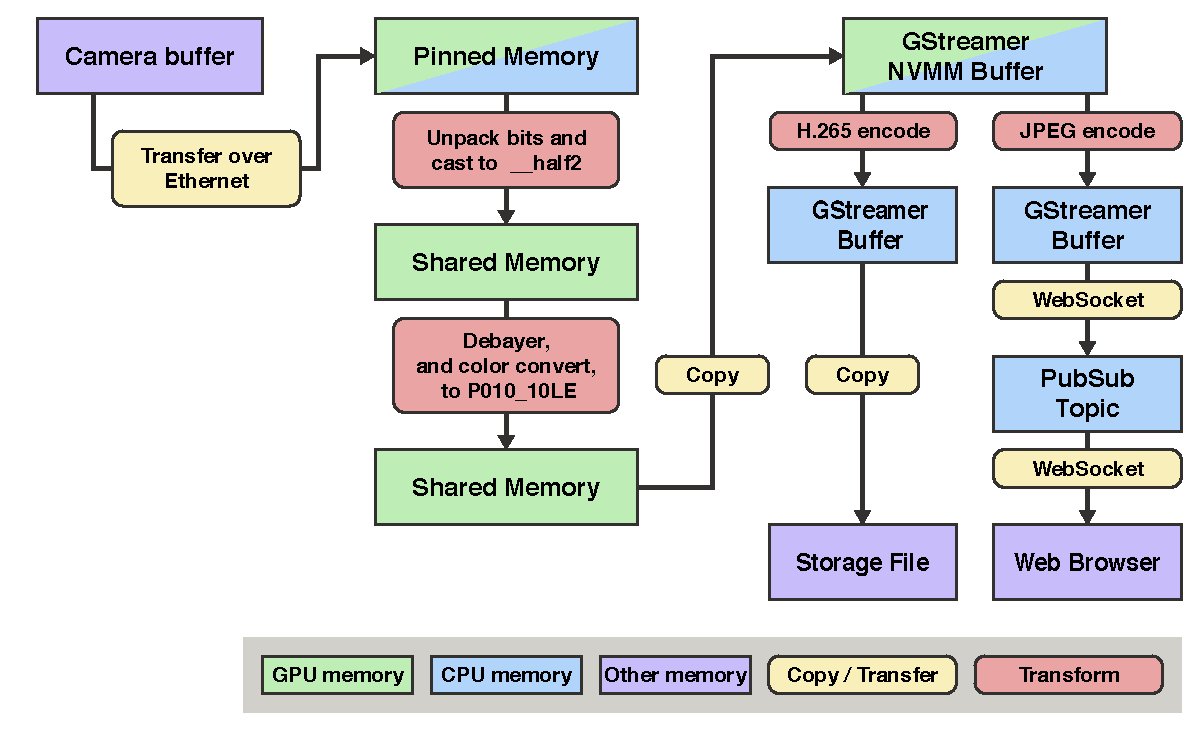
\includegraphics[width=\textwidth]{figures/memory_pipeline/optimal.pdf}
    \caption{Overview of the memory pipeline}
    \label{fig:pipeline_optimal}
\end{figure}